\documentclass{beamer}

%
% Choose how your presentation looks.
%
% For more themes, color themes and font themes, see:
% http://deic.uab.es/~iblanes/beamer_gallery/index_by_theme.html
%
\mode<presentation>
{
  \usetheme{default}      % or try Darmstadt, Madrid, Warsaw, ...
  \usecolortheme{default} % or try albatross, beaver, crane, ...
  \usefonttheme{default}  % or try serif, structurebold, ...
  \setbeamertemplate{navigation symbols}{}
  \setbeamertemplate{caption}[numbered]
  \setbeamertemplate{footline}[page number]
  \setbeamercolor{frametitle}{fg=white}
  \setbeamercolor{footline}{fg=black}
} 

\usepackage[english]{babel}
\usepackage[utf8x]{inputenc}
\usepackage{tikz}
\usepackage{listings}
\usepackage{courier}
\usepackage{minted}

\xdefinecolor{darkblue}{rgb}{0.1,0.1,0.7}
\xdefinecolor{darkgreen}{rgb}{0,0.5,0}
\xdefinecolor{darkorange}{rgb}{0.8,0.5,0}
\xdefinecolor{darkred}{rgb}{0.7,0,0}
\xdefinecolor{dianablue}{rgb}{0.18,0.24,0.31}
\definecolor{commentgreen}{rgb}{0,0.6,0}
\definecolor{stringmauve}{rgb}{0.58,0,0.82}

\lstset{ %
  backgroundcolor=\color{white},      % choose the background color
  basicstyle=\ttfamily\small,         % size of fonts used for the code
  breaklines=true,                    % automatic line breaking only at whitespace
  captionpos=b,                       % sets the caption-position to bottom
  commentstyle=\color{commentgreen},  % comment style
  escapeinside={\%*}{*)},             % if you want to add LaTeX within your code
  keywordstyle=\color{blue},          % keyword style
  stringstyle=\color{stringmauve},    % string literal style
  showstringspaces=false,
  showlines=true
}

\lstdefinelanguage{scala}{
  morekeywords={abstract,case,catch,class,def,%
    do,else,extends,false,final,finally,%
    for,if,implicit,import,match,mixin,%
    new,null,object,override,package,%
    private,protected,requires,return,sealed,%
    super,this,throw,trait,true,try,%
    type,val,var,while,with,yield},
  otherkeywords={=>,<-,<\%,<:,>:,\#,@},
  sensitive=true,
  morecomment=[l]{//},
  morecomment=[n]{/*}{*/},
  morestring=[b]",
  morestring=[b]',
  morestring=[b]"""
}

\title[2016-12-12-femtocode-at-diana]{Femtocode: development of a query \\ language for HEP}
\author{Jim Pivarski}
\institute{Princeton -- DIANA}
\date{December 12, 2016}

\begin{document}

\logo{\pgfputat{\pgfxy(0.11, 8)}{\pgfbox[right,base]{\tikz{\filldraw[fill=dianablue, draw=none] (0 cm, 0 cm) rectangle (50 cm, 1 cm);}}}\pgfputat{\pgfxy(0.11, -0.6)}{\pgfbox[right,base]{\tikz{\filldraw[fill=dianablue, draw=none] (0 cm, 0 cm) rectangle (50 cm, 1 cm);}
\includegraphics[height=0.99 cm]{diana-hep-logo.png}\tikz{\filldraw[fill=dianablue, draw=none] (0 cm, 0 cm) rectangle (4.9 cm, 1 cm);}}}}

\begin{frame}
  \titlepage
\end{frame}

\logo{\pgfputat{\pgfxy(0.11, 8)}{\pgfbox[right,base]{\tikz{\filldraw[fill=dianablue, draw=none] (0 cm, 0 cm) rectangle (50 cm, 1 cm);}
\includegraphics[height=1 cm]{diana-hep-logo.png}}}}

% Uncomment these lines for an automatically generated outline.
%\begin{frame}{Outline}
%  \tableofcontents
%\end{frame}

\begin{frame}{Motivations}
\textcolor{darkblue}{\underline{Specific motivation}: to accelerate data pulls, both}

\begin{center}
\begin{columns}
\column{0.1\linewidth}

\column{0.28\linewidth}
\centering \textcolor{darkblue}{for the humans}

{\it shorter time from concept to code}

\column{0.05\linewidth}
\centering \textcolor{darkblue}{and}

\column{0.28\linewidth}
\centering \textcolor{darkblue}{for the computers.}

{\it shorter time from code to results}

\column{0.1\linewidth}
\end{columns}
\end{center}

\vspace{0.2 cm}
\textcolor{gray}{(By ``data pull,'' I mean extract, transform, and filter data from a collaboration's central dataset (AOD) and download it for further processing. Right now, we're writing C++ modules.)}

\vspace{0.5 cm}
\begin{uncoverenv}<2->
\textcolor{darkblue}{``\underline{Chip on my shoulder}''}

\vspace{0.2 cm}
To show that a very high-level, abstract view of computation can nevertheless be fast.
\end{uncoverenv}
\end{frame}

\begin{frame}[fragile]{High-level and speed are not antithetical}
\vspace{0.5 cm}
\begin{columns}
\column{0.55\linewidth}
Code like

\small
\begin{minted}{scala}
bestmuon =
  muons.filter(m => m.iso > 10)
       .maxBy(m => m.pt)
\end{minted}
\vspace{0.4 cm}

\column{0.35\linewidth}
\\ does {\it not} need to create function objects or muon objects at runtime!

\vspace{0.2 cm}
It need not be ``taken literally.''
\end{columns}

\vspace{0.5 cm}
\textcolor{darkblue}{Another possible execution plan:}
\begin{enumerate}
\item Start with all {\tt\small muon.iso} values in one array, all {\tt\small muon.pt} values in another array, and a ``repetition level'' to specify where events begin and end.
\item Apply the contents of the filter function to make a mask.
\item Use the mask and repetition level to compact the {\tt\small muon.pt} into zero or one results per event.
\end{enumerate}
\end{frame}

\begin{frame}{How fast {\it should} it be?}
\vspace{0.3 cm}
\textcolor{darkorange}{\bf Suppose we want to plot all CMS $t\bar{t}$ data ever collected.}
\begin{itemize}
\item About 100~fb$^{-1}$ (\href{http://cms-service-lumi.web.cern.ch/cms-service-lumi/publicplots/int_lumi_cumulative_pp_1.png}{\textcolor{blue}{plot}}) $\times$ 1~nb (\href{https://atlas.web.cern.ch/Atlas/GROUPS/PHYSICS/CombinedSummaryPlots/SM/ATLAS_p_SMSummary_SqrtS_Zoom/ATLAS_p_SMSummary_SqrtS_Zoom.png}{\textcolor{blue}{plot}}) is 100 million events.
\item Derivation of a plotted quantity could involve $\mathcal{O}(100)$ double-precision values per event.
\item That's only 80~GB of data that needs to be evaluated; anything else is overhead.
\end{itemize}

\vspace{0.5 cm}
\textcolor{darkblue}{{\it \underline{Single}} computer, {\it \underline{single}} thread:}

\vspace{0.1 cm}
\begin{description}
\item[load from disk:] 21 minutes (Numpy), 22 minutes (ROOT)
\item[CPU execution:] 70 seconds (no optimization), 13 seconds ({\tt -O3})
\item[GPU execution:] 12 seconds to copy to GPU, 5 seconds to compute
\end{description}

\vspace{0.1 cm}
\textcolor{gray}{(Probably close to ``theoretical optimum.'' Distributed processing and multi-user cache can help.)}
\end{frame}

\begin{frame}{Role of language}
\vspace{0.5 cm}
Directly filling histograms from the collaboration-wide repository, eliminating private skims, would fundamentally improve analysis workflows. Analysis could become ``interactive.''

\vspace{0.5 cm}
\textcolor{darkblue}{But\ldots\ how can a language help?}

\begin{uncoverenv}<2->
\vspace{0.3 cm}
\begin{itemize}
\item Writing vectorized, one-array-at-a-time algorithms is unnatural, distracting from analysis.
\item Physicists {\it should} be thinking about one event at a time and muons as objects.
\end{itemize}

\vspace{0.3 cm}
\textcolor{darkblue}{Transforming human concepts into physical execution is exactly what programming languages are for.}
\end{uncoverenv}
\end{frame}

\begin{frame}{What's wrong with the languages we have?}
\vspace{0.25 cm}
As I said in \href{https://indico.cern.ch/event/544650/}{\textcolor{blue}{my June 20 talk}}, C++ and Python are too expressive to permit these kinds of optimizations.

\vspace{0.5 cm}
Automatic vectorization is (in general) an unsolved problem in computer science. But building a vectorizable language is relatively easy: they're just less capable. Typically, query languages like SQL are vectorized.

\vspace{0.5 cm}
Business intelligence with SQL is typically ``interactive,'' and big data projects are pushing $\mathcal{O}(\mbox{second})$ response times to petabyte scales: Ibis, Impala, Kudu, Drill, \ldots\ others? (\href{http://research.google.com/pubs/pub36632.html}{\textcolor{blue}{Google paper}}).

\vspace{0.5 cm}
\textcolor{darkorange}{\bf However, SQL and its relatives are not sufficient for us.}
\end{frame}

\begin{frame}[fragile]{Nested query in C++}
\vspace{0.5 cm}
{\bf Example query:}
\begin{center}
\begin{minipage}{0.95\linewidth}
\textcolor{darkblue}{``Momentum of the track with $|\eta|$ $<$ 2.4 that has the most hits.''}
\end{minipage}
\end{center}
\small
\begin{minted}{c++}
Track *best = NULL;
for (int i = 0;  i < tracks.size();  i++) {
  if (fabs(tracks[i]->eta) < 2.4)
    if (best == NULL ||
        tracks[i]->hits.size() > best->hits.size())
      best = tracks[i];
}
if (best != NULL)
  return best->pt;
else
  return 0.0;
\end{minted}
\end{frame}

\begin{frame}[fragile]{Nested query in SQL}
\vspace{0.5 cm}
{\bf Example query:}
\begin{center}
\begin{minipage}{0.95\linewidth}
\textcolor{darkblue}{``Momentum of the track with $|\eta|$ $<$ 2.4 that has the most hits.''}
\end{minipage}
\end{center}
\small
\begin{minted}{sql}
WITH hit_stats AS (
  SELECT hit.track_id, COUNT(*) AS hit_count FROM hit
    GROUP BY hit.track_id),
 track_sorted AS (
    SELECT track.*, 
    ROW_NUMBER() OVER (
     PARTITION BY track.event_id
     ORDER BY hit_stats.hit_count DESC)
  track_ordinal FROM track INNER JOIN hit_stats
    ON hit_stats.track_id = track.id
    WHERE ABS(track.eta) < 2.4)
 SELECT * FROM event INNER JOIN track_sorted
   ON track_sorted.event_id = event.id
WHERE
  track_sorted.track_ordinal = 1
\end{minted}
\end{frame}

\begin{frame}[fragile]{Nested query in Femtocode}
\vspace{0.5 cm}
{\bf Example query:}
\begin{center}
\begin{minipage}{0.95\linewidth}
\textcolor{darkblue}{``Momentum of the track with $|\eta|$ $<$ 2.4 that has the most hits.''}
\end{minipage}
\end{center}
\small
\begin{onlyenv}<1>
\begin{minted}{bash}
tracks.filter(t => abs(t.eta) < 2.4)   # drop tracks
      .maxBy(t => t.hits.size)   # pick one (if any)
      .map(t => t.pt)            # transform it
      .impute(0.0)               # replace "None"
                                 # with a value
\end{minted}
\end{onlyenv}
\begin{onlyenv}<2>
\begin{minted}{bash}
tracks.filter(abs($1.eta) < 2.4)       # drop tracks
      .maxBy($1.hits.size)       # pick one (if any)
      .map($1.pt)                # transform it
      .impute(0.0)               # replace "None"
                                 # with a value
\end{minted}
\end{onlyenv}
\end{frame}

\begin{frame}[fragile]{Femtocode: tiny, declarative code snippets}
\vspace{0.4 cm}
Combine the {\it implementation flexibility} of declarative languages like SQL with the {\it expressiveness} of a functional language for dealing with nested structure.

\vspace{0.5 cm}
{\bf Example use in Python:}

\small
\begin{minted}{python}
h = db.dataset("ttbar-MC")
  .withColumn(varName = "<Femtocode goes here>")
  .filter("<Femtocode using varName>")
  .flatMap("<Femtocode changing nesting level>")
  .Label(hist1 = Bin(100, -5.0, 5.0, "<Femtocode>"),
         hist2 = Bin(20, 0.0, 100.0, "<Femtocode>"),
         hist3 = Bin(314, -pi, pi, "<Femtocode>"))
\end{minted}

\normalsize
followed by Python analysis on {\small\tt h[\textcolor{darkred}{"hist1"}]}, {\small\tt h[\textcolor{darkred}{"hist2"}]}\ldots

\vspace{0.1 cm}
\begin{uncoverenv}<2->
\textcolor{darkblue}{Python manipulates streams of events and accepts the output, while Femtocode (in quotes) operates on individual events.}

\vspace{0.1 cm}
Integrates with Histogrammar ({\tt\small Label}, {\tt\small Bin}) to aggregate result.
\end{uncoverenv}
\end{frame}

\begin{frame}[fragile]{Working examples}
\vspace{0.3 cm}
\begin{lstlisting}[language=python]
>>> from femtocode.parser import parse
>>> print ast.dump(parse("""
... tracks.filter(abs($1.eta) < 2.4)
...       .maxBy($1.hits.size)
...       .map($1.pt)
...       .impute(0.0)
... """))
\end{lstlisting}
\begin{lstlisting}[language=python,basicstyle=\ttfamily\scriptsize]
Suite(assignments=[], expression=FcnCall(function=Attribute(value=FcnCall(function=Attribute(value=FcnCall(function=Attribute(value=FcnCall(function=Attribute(value=Name(id='tracks', ctx=Load()), attr='filter', ctx=Load()), positional=[Compare(left=FcnCall(function=Name(id='abs', ctx=Load()), positional=[Attribute(value=AtArg(num=1), attr='eta', ctx=Load())], names=[], named=[]), ops=[Lt()], comparators=[Num(n=2.4)])], names=[], named=[]), attr='maxBy', ctx=Load()), positional=[Attribute(value=Attribute(value=AtArg(num=1), attr='hits', ctx=Load()), attr='size', ctx=Load())], names=[], named=[]), attr='map', ctx=Load()), positional=[Attribute(value=AtArg(num=1), attr='pt', ctx=Load())], names=[], named=[]), attr='impute', ctx=Load()), positional=[Num(n=0.0)], names=[], named=[]))
\end{lstlisting}
\end{frame}

\begin{frame}[fragile]{Working examples}
\vspace{0.3 cm}
\begin{lstlisting}[language=python]
>>> propagateTypes("""
... data.map(x => x + y)
... """,
... data=collection(integer), y=integer)
collection(integer)
\end{lstlisting}

\begin{lstlisting}[language=python]
>>> propagateTypes("""
... data.map(x => x + y)
... """,
... data=collection(integer), y=real)
collection(real)
\end{lstlisting}

\begin{lstlisting}[language=python]
>>> propagateTypes("""
... data.map(x => x + y)
... """,
... data=collection(integer, fewest=10, most=10),
... y=integer)
collection(integer, fewest=10, most=10)
\end{lstlisting}
\end{frame}

\begin{frame}[fragile]{Working examples}
\vspace{0.3 cm}
\textcolor{darkblue}{Propagate intervals of validity:}
\begin{lstlisting}[language=python]
>>> propagateTypes("""
... data.map(x => x + y)
... """,
... data=collection(real(min=3, max=5)),
... y=real(min=100, max=200))
collection(real(min=103.0, max=205.0))
\end{lstlisting}

\vfill
\textcolor{darkblue}{Properly handle shadowed variable ``x'':}
\begin{lstlisting}[language=python]
>>> propagateTypes("""
... y = x + -100;
... data.map(x => x + y)
... """,
... data=collection(real(min=3, max=5)),
... x=real(min=100, max=200))
collection(real(min=3.0, max=105.0))
\end{lstlisting}
\end{frame}

\begin{frame}{Type system is highly granular}
\vspace{0.5 cm}
Collections have \textcolor{darkblue}{fewest} and \textcolor{darkblue}{most} number of elements, and numbers have \textcolor{darkblue}{min} and \textcolor{darkblue}{max} intervals:
\begin{itemize}
\item {\tt\small real(almost(0), 10)} \hfill $\{x | x \in \mathbb{R}\mbox{ and } 0 < x \le 10\}$
\item {\tt\small integer(almost(-inf), almost(inf))} \hfill $\mathbb{Z}$
\item {\tt\small extended(-inf, inf)} \hfill $\mathbb{R} \cup \{-\infty, \infty\}$
\item {\tt\small union(integer, real(0))} \hfill $\mathbb{Z} \cup \{x | x \in \mathbb{R}\mbox{ and } x \ge 0\}$
\end{itemize}

\vfill
\begin{uncoverenv}<2->
\textcolor{darkorange}{\bf Why?}

\vspace{0.2 cm}
To eliminate the possibility of runtime errors.

\vspace{0.2 cm}
With enough information in the type system, the compiler can identify runtime errors before submitting the job, saving the author time and protecting shared resources from waste.

\vspace{0.2 cm}
\textcolor{gray}{(Someday, they might be cloud-based and cost real money.)}
\end{uncoverenv}
\end{frame}

\begin{frame}[fragile]{Working examples}
\vspace{0.2 cm}
\begin{lstlisting}[language=python]
>>> propagateTypes("x / y", x=real, y=real)
\end{lstlisting}
\color{red}
\begin{lstlisting}[basicstyle=\ttfamily\scriptsize]
femtocode.parser.FemtocodeError: Function "/" does not accept arguments with the given types:

    /(real,
      real)

    Indeterminate form (0 / 0) is possible; constrain with if-else.

Check line:col 1:0 (pos 0):

    x / y
----^
\end{lstlisting}

\textcolor{darkblue}{Applying a constraint changes the type of ``y'' in the ``if'' clause to {\tt\small union(real(max=almost(0)), real(min=almost(0)))}.}
\color{black}
\begin{lstlisting}[language=python]
>>> propagateTypes("if y != 0: x / y else: None",
...     x=real, y=real)
union(null, real)
\end{lstlisting}
\end{frame}

\begin{frame}[fragile]{Working examples}
\vspace{0.5 cm}
\begin{onlyenv}<1>
\textcolor{darkblue}{``if'', ``and'', ``or'', and ``not'' propagate constraints.}
\begin{lstlisting}[language=python]
>>> propagateTypes("x == 5 and y == 6 and x == y",
... x=real, y=real)
\end{lstlisting}
\color{red}
\begin{lstlisting}[basicstyle=\ttfamily\scriptsize]
femtocode.parser.FemtocodeError: Function "==" does not accept arguments with the given types:

    ==(integer(min=5, max=5),
       integer(min=6, max=6))

    The argument types have no overlap (values can never be equal).

Check line:col 1:27 (pos 27):

    x == 5 and y == 6 and x == y
-------------------------------^
\end{lstlisting}
\end{onlyenv}
\begin{onlyenv}<2->
\textcolor{darkblue}{Order does not matter.}
\begin{lstlisting}[language=python]
>>> propagateTypes("x == y and x == 5 and y == 6",
... x=real, y=real)
\end{lstlisting}
\color{red}
\begin{lstlisting}[basicstyle=\ttfamily\scriptsize]
femtocode.parser.FemtocodeError: Function "==" does not accept arguments with the given types:

    ==(integer(min=5, max=5),
       integer(min=6, max=6))

    The argument types have no overlap (values can never be equal).

Check line:col 1:5 (pos 5):

    x == y and x == 5 and y == 6
---------^
\end{lstlisting}
\end{onlyenv}

\uncover<3>{\textcolor{gray}{(It's a short step from here to simplifying the algebra with SymPy.)}}
\end{frame}

\begin{frame}[fragile]{Working examples}
\begin{onlyenv}<1>
\begin{lstlisting}[language=python]
>>> viewAsTree("""
... a = x + y;
... b = a + y + z;
... xs.map(x => x + a + a + b).map(y => y + 2)""",
... xs=collection(real), x=real, y=real, z=real)
\end{lstlisting}
\end{onlyenv}
\begin{onlyenv}<2>
\begin{lstlisting}[language=python]
>>> viewAsStatements("""
... a = x + y;
... b = a + y + z;
... xs.map(x => x + a + a + b).map(y => y + 2)""",
... xs=collection(real), x=real, y=real, z=real)
\end{lstlisting}
\end{onlyenv}

\vspace{-0.5 cm}
\begin{minipage}[t][12cm][t]{\textwidth}
\begin{onlyenv}<1>
\begin{lstlisting}[basicstyle=\ttfamily\tiny]
Call BuiltinFunction[".map"] has type collection(real)
    Call BuiltinFunction[".map"] has type collection(real)
        Ref xs (frame None) has type collection(real)
        UserFunction has type real
            Call BuiltinFunction["+"] has type real
                Call BuiltinFunction["+"] has type real
                    Call BuiltinFunction["+"] has type real
                        Ref x (frame 2) has type real
                        Call BuiltinFunction["+"] has type real
                            Ref x (frame None) has type real
                            Ref y (frame None) has type real
                    Call BuiltinFunction["+"] has type real
                        Ref x (frame None) has type real
                        Ref y (frame None) has type real
                Call BuiltinFunction["+"] has type real
                    Call BuiltinFunction["+"] has type real
                        Call BuiltinFunction["+"] has type real
                            Ref x (frame None) has type real
                            Ref y (frame None) has type real
                        Ref y (frame None) has type real
                    Ref z (frame None) has type real
    UserFunction has type real
        Call BuiltinFunction["+"] has type real
            Ref y (frame 3) has type real
            Literal 2 has type integer(min=2, max=2)
\end{lstlisting}
\vspace{-6 cm}
\mbox{ } \hfill Notice that ``a'' and

\mbox{ } \hfill ``b'' do not appear.

\vspace{6 cm}
\end{onlyenv}
\begin{onlyenv}<2>
\begin{lstlisting}[basicstyle=\ttfamily\small]
tmp_0 := (+ x y)
tmp_1 := (+ xs tmp_0)
tmp_2 := (+ x y)
tmp_3 := (+ tmp_1 tmp_2)
tmp_4 := (+ x y)
tmp_5 := (+ tmp_4 y)
tmp_6 := (+ tmp_5 z)
tmp_7 := (+ tmp_3 tmp_6)
tmp_8 := (+ tmp_7 2)
\end{lstlisting}
\vspace{-3.7 cm}
\normalsize
\mbox{ } \hfill Repeated calculations have

\mbox{ } \hfill been rolled into {\tt\small tmp\_*}.

\vspace{3.7 cm}
\end{onlyenv}
\end{minipage}
\end{frame}

\begin{frame}{Status and plans}
\vspace{0.3 cm}
\textcolor{darkblue}{Done:}
\begin{itemize}
\item Syntax, parsing, abstract syntax tree.
\item Type system, type propagation, type inference for {\tt +}, {\tt -}, {\tt *}, {\tt /}, {\tt //}, {\tt **}, {\tt \%}.
\item Type constraints in ``if'', ``and'', ``or'', and ``not''.
\item Prototype for generating statements.
\end{itemize}

\vfill
\textcolor{darkblue}{To do:}
\begin{itemize}
\item Fully generate statements and evaluate on arrays.
\item Implement a few more functions for basic usability.
\item Focus-group the syntax and scope: will this work for busy physicists?
\item Get more feedback from Brian, Philippe, and other experts.
\item Work with Jin Chang and Igor Mandrichenko on server.
\item Discuss with ROOT Team about value as a ROOT 7 TTreeFormula replacement.
\end{itemize}
\end{frame}

\begin{frame}{}
\begin{center}
\textcolor{darkblue}{\huge BACKUP}
\end{center}
\end{frame}

\begin{frame}{Features of Femtocode}
\vspace{0.5 cm}
\begin{description}
\item[Declarative:] order written/order evaluated need not be the same.
\item[Functional:] map/filter/maxBy instead of explicit for loops.
\item[Vectorizable:] code appears to act on rows (e.g.\ events), but automatically translated to operate on columns.
\item[No unbounded loops:] execution time strictly scales with input data size; not Turing complete.
\item[No runtime errors:] any compilable query will return some result.
\item[Statically typed:] stronger type system than most languages is needed to eliminate runtime errors.
\item[Full type inference:] explicitly writing down types is annoying.
\item[No recursion:] combining recursion with \textcolor{darkblue}{no unbounded loops} is complicated, but big data pulls don't need recursion.
\item[Pythonic syntax:] familiar to physics users; don't invent new syntax unless absolutely necessary.
\end{description}
\end{frame}

\begin{frame}[fragile]{Syntax}
\vspace{0.25 cm}
\textcolor{darkblue}{BNF specification of Femtocode syntax} \only<2->{\textcolor{red}{that is identical to Python}}

\vspace{-0.5 cm}
\begin{columns}[t]
\column{0.5\linewidth}
\tiny
\begin{verbatim}body: ';'* suite
suite: (assignment ';'*)* expression ';'*
lvalues: (NAME ',')* NAME [',']
assignment: (lvalues '=' closed_expression
              | fcnndef)
fcnndef: ('def' NAME '(' [paramlist] ')'
            closed_exprsuite)
expression: ifblock | fcndef | or_test
closed_expression: (closed_ifblock | fcndef
                     | or_test ';')
fcndef: '{' [paramlist] '=>' ';'* suite '}'
fcn1def: parameter '=>' expression
paramlist: (parameter ',')* (parameter [','])
parameter: NAME ['=' expression]
exprsuite: (':' expression
             | [':'] '{' ';'* suite '}')
closed_exprsuite: (':' closed_expression
             | [':'] '{' ';'* suite '}')
ifblock: ('if' expression exprsuite
            ('elif' expression exprsuite)*
             'else' exprsuite)
closed_ifblock: ('if' expression exprsuite
            ('elif' expression exprsuite)*
             'else' closed_exprsuite)
\end{verbatim}
\vspace{-0.8 cm}\only<2->{\color{red}}
\begin{verbatim}or_test: and_test ('or' and_test)*
and_test: not_test ('and' not_test)*
not_test: 'not' not_test | comparison
comparison: typecheck (comp_op typecheck)*
comp_op: ('<' | '>' | '==' | '>=' | '<='
              | '!=' | 'in' | 'not' 'in')
\end{verbatim}

\column{0.5\linewidth}
\tiny\only<2->{\color{black}}
\begin{verbatim}typecheck: (arith_expr ['is' arith_expr
             | 'is' 'not' arith_expr])
\end{verbatim}
\vspace{-0.8 cm}\only<2->{\color{red}}
\begin{verbatim}arith_expr: term (('+' | '-') term)*
term: factor (('*' | '/' | '%' | '//') factor)*
factor: ('+' | '-') factor | power
power: atom trailer* ['**' factor]
atom: ('(' expression ')'
\end{verbatim}
\vspace{-0.8 cm}\only<2->{\color{black}}
\begin{verbatim}      | ('[' (expression ',')*
             [expression [',']] ']')
       | fcndef '(' [arglist] ')'
\end{verbatim}
\vspace{-0.8 cm}\only<2->{\color{red}}
\begin{verbatim}      | MULTILINESTRING
       | STRING
       | IMAG_NUMBER
       | FLOAT_NUMBER
       | HEX_NUMBER
       | OCT_NUMBER
       | DEC_NUMBER
\end{verbatim}
\vspace{-0.8 cm}\only<2->{\color{black}}
\begin{verbatim}      | ATARG
\end{verbatim}
\vspace{-0.8 cm}\only<2->{\color{red}}
\begin{verbatim}      | NAME)
trailer: ('(' [arglist] ')'
           | '[' subscriptlist ']' | '.' NAME)
subscriptlist: subscript (',' subscript)* [',']
subscript: (expression
           | [expression] ':' [expression]
             [sliceop])
sliceop: ':' [expression]
\end{verbatim}
\vspace{-0.8 cm}\only<2->{\color{black}}
\begin{verbatim}arglist: (((argument ',')* (argument [',']))
           | fcn1def)
argument: expression | NAME '=' expression
\end{verbatim}
\end{columns}
\end{frame}

\begin{frame}[fragile]{Syntax}
\vspace{0.3 cm}
\begin{columns}[t]
\column{0.5\linewidth}
\textcolor{darkblue}{\underline{\bf How is it like Python?}}
\begin{itemize}
\item mathematical expressions and operator precedence:

{\small\tt (-b + sqrt(b**2 -

\hfill 4*a*c))/(2*a)}

\item slices and 0-indexing:

{\small\tt lheweights[::2]}

\item numbers and string literals (favoring Python 3):

{\small\tt 0xff, 0o77, .3e7, 1j,

"""multi \textbackslash"line\textbackslash"

string"""}

\item chained comparisons:

{\small\tt 0 < x <= 10}

\item keyword arguments:

{\small\tt f(arg, some=kwd)}

\end{itemize}

\column{0.5\linewidth}
\textcolor{darkblue}{\underline{\bf How is it different?}}
\begin{itemize}
\item anonymous functions:

{\small\tt \{x, y => x + y\}

\{\$1 + \$2\}}

\item no statements and whitespace independent:

{\small\tt if something:

\ \ \ doIfTrue()

\ \ \ else:

\ doIfFalse()}

\item curly-bracketed blocks with semicolon-separated assignments ending in a single expression.

{\small\tt if something \{doIfTrue()\} else \{doIfFalse()\}}
\end{itemize}
\end{columns}
\end{frame}

\begin{frame}{Abstract type system}
\vspace{0.5 cm}
Space of possible datasets is defined by the type system.

\begin{description}
\item[null:] type with only one value
\item[boolean:] not the same as integers
\item[number:] further defined by attributes: \textcolor{darkblue}{min}, \textcolor{darkblue}{max}, \textcolor{darkblue}{whole}

{\tt whole == True} means integer,

{\tt whole == False} means floating point

\item[string:] \textcolor{darkblue}{charset} (``bytes'' or ``unicode''), \textcolor{darkblue}{fewest}, \textcolor{darkblue}{most};

\textcolor{darkblue}{fewest/most} constrain the string length

\item[collection:] \textcolor{darkblue}{fewest}, \textcolor{darkblue}{most}, \textcolor{darkblue}{ordered}

fixed-size arrays/matrices have {\tt fewest == most and ordered == True}

\item[record:] defined by a dictionary of \textcolor{darkblue}{fields}
\item[union:] tagged union, such as {\tt union(null, string)} for a nullable string type.
\end{description}
\end{frame}

\begin{frame}{Semantics}
Every Femtocode ``program'' is conceptually a single expression: that which should be computed from the input fields.
\begin{itemize}
\item when called in a {\tt filter}, it selects events,
\item in {\tt map}, it transforms,
\item in {\tt flatMap}, it restructures,
\item in {\tt withColumn}, it adds a field to the output,
\item in Histogrammar quantities, it gets aggregated, probably for plotting.
\end{itemize}

\vspace{0.5 cm}
Most Femtocode snippets are small enough for this to be obvious!
\end{frame}

\begin{frame}[fragile]{Semantics}
\vspace{0.5 cm}
Assignments are provided {\it as a convenience.}

\begin{center}
\begin{minipage}{0.9\linewidth}
\small
\begin{lstlisting}[language=python]
goodVertex = abs(z) < 3;
goodPt = pt > 20;
goodIsolation = iso > 12;
goodVertex and goodPt and goodIsolation
\end{lstlisting}
\end{minipage}
\end{center}

Expression ASTs are literally inserted where they are referenced \textcolor{gray}{(handling shadowed variable names appropriately, with lexical scope)}.

\vspace{0.5 cm}
This is legal because Femtocode has perfect referential transparency. \textcolor{gray}{(All variables are immutable, no side-effects, no exceptions or non-halting functions.)}
\end{frame}

\begin{frame}[fragile]{Semantics}
\vspace{0.5 cm}
The same is true of user-defined functions. Moreover, arguments might have different types in different calls.

\begin{center}
\begin{minipage}{0.9\linewidth}
\small
\begin{lstlisting}[language=python]
def nonempty(x) {
  x.size > 0
}

nonempty(list) or nonempty(str)
\end{lstlisting}
\end{minipage}
\end{center}

When applied to a collection, {\small\tt nonempty} takes the collection type, when applied to a string, {\small\tt nonempty} takes the string type.

\vspace{0.5 cm}
Types are propagated independently through the function's body with each call. (Thus, it deals with ugly unions transparently.)

\vspace{0.5 cm}
\textcolor{gray}{(This is what Julia does when you don't provide type annotations.)}
\end{frame}

\begin{frame}[fragile]{Semantics}
So what about recursion? What's its type?

\begin{center}
\begin{minipage}{0.9\linewidth}
\small
\begin{lstlisting}[language=python]
def listsum(x) {
  if nonempty(x):
    x[0] + listsum(x[1:])
  else:
    0
}

listsum(list)
\end{lstlisting}
\end{minipage}
\end{center}

It can't always be determined, and we want to eliminate infinite loops anyway, so we simply don't allow recursion.
\end{frame}

\begin{frame}[fragile]{Semantics}
The rule against recursion applies equally to assignment (like a zero-argument function).

\begin{center}
\begin{minipage}{0.9\linewidth}
\small
\begin{lstlisting}[language=python]
x = x + 1
\end{lstlisting}
\end{minipage}
\end{center}

\textcolor{gray}{(If we attempted to interpret the above, we'd have to conclude that {\tt x} is {\tt inf} or {\tt -inf}. Probably not what the user intended.)}
\end{frame}

\begin{frame}[fragile]{Semantics}
\vspace{0.5 cm}
Although not logically necessary, we require values and functions to be defined before they are used.

\begin{center}
\begin{minipage}{0.9\linewidth}
\small
\begin{lstlisting}[language=python]
goodParticle = goodVertex and goodPt and goodIsolation;
goodVertex = abs(z) < 3;
goodPt = pt > 20;
goodIsolation = iso > 12;
\end{lstlisting}
\hspace{-0.6 cm} and
\begin{lstlisting}[language=python]
def invmass(p4): sqrt(energy(p4)**2 - momentum(p4)**2);
def energy(p4): p4[0];
def momentum(p4): sqrt(p4[1]**2 + p4[2]**2 + p4[3]**2);
\end{lstlisting}
\end{minipage}
\end{center}

are not allowed. The first would likely be a user mistake.
\end{frame}

\begin{frame}[fragile]{Second-class functions}
\vspace{0.5 cm}
In some languages, functions are ``first class'' (in the sense of ``first class citizens'') because they can be treated as values, just like numbers or strings. Femtocode is not such a language.

\vspace{0.5 cm}
\begin{uncoverenv}<2->
After all assignments have been expanded, anonymous functions and function names can only appear in the arguments of built-in functions that expect them.

\begin{center}
\begin{minipage}{0.9\linewidth}
\small
\begin{minted}{python}
def goodEta(t): abs(t.eta) < 2.4;
tracks.filter(goodEta)
      .maxBy(t => t.hits.size)
      .map($1.pt)
\end{minted}
\end{minipage}
\end{center}

{\tt goodEta}, {\tt t => t.hits.size}, and {\tt \$1.pt} can only appear in the appropriate argument slot of functions like {\tt .filter}, {\tt .maxBy}, and {\tt .map}.

\vspace{0.5 cm}
And built-in functions never return functions.
\end{uncoverenv}
\end{frame}

\begin{frame}[fragile]{Second-class functions}
\vspace{0.5 cm}
However, functions can be assigned
\begin{center}
\begin{minipage}{0.9\linewidth}
\small
\begin{lstlisting}[language=scala]
goodEta = {t => abs(t.eta) < 2.4};
\end{lstlisting}
\end{minipage}
\end{center}
and passed as the return value of a user-defined function
\begin{center}
\begin{minipage}{0.9\linewidth}
\small
\begin{lstlisting}[language=scala]
def cutEta(cut):
  {t => abs(t.eta) < cut};
goodEta = cutEta(2.4);
\end{lstlisting}
\end{minipage}
\end{center}
because these constructs are expanded before any types are checked. It gives the user the feeling of freedom when working with functions when they are actually constrained.

\vspace{0.5 cm}
The only aspect of first-class functions that the user might miss is the ability to pick a function to call at runtime.
\end{frame}

\begin{frame}[fragile]{Why does this matter?}
\vspace{0.5 cm}
Since unevaluated functions only appear in arguments to {\tt .filter}, {\tt .maxBy}, and {\tt .map}, etc., they are no more powerful than a ``for'' loop body.

\vspace{0.25 cm}
For instance,
\begin{center}
\begin{minipage}{0.9\linewidth}
\small
\begin{lstlisting}[language=python]
goodEta = {t => abs(t.eta) < 2.4};
data.filter(goodEta)
\end{lstlisting}
\end{minipage}
\end{center}
could be implemented by
\begin{center}
\begin{minipage}{0.9\linewidth}
\small
\begin{minted}{python}
[t for t in data if abs(t.eta) < 2.4]
\end{minted}
\end{minipage}
\end{center}
In C terminology, all functions can be ``inlined.'' That is to say, the exact code needed to execute them is known at compile-time and can be literally inserted if desired.
\end{frame}

\begin{frame}{Vectorization}
\vspace{0.5 cm}
It is in general difficult to ``vectorize'' code: that is, convert code that operates on individual rows of data (events) to instead operate on columns.
\begin{itemize}
\item The row-based view is more natural to the data analyst.
\item But the column-based implementation is often faster.
\end{itemize}

\vspace{0.5 cm}
\begin{uncoverenv}<2->
This is the difficulty of porting algorithms from CPU to GPU: the GPU is a 32 or 64 lane wide vector machine.

\vspace{0.2 cm}
\textcolor{gray}{It is also the difficulty of porting pure Python to Numpy. Or ``for'' loops in R into efficient ``lapply.''}

\vspace{0.5 cm}
Even when the CPU is the target, modern CPUs have $\sim$4 lane wide vector registers and can prefetch memory better when operating on columns (circumventing the primary bottleneck in most calculations).
\end{uncoverenv}
\end{frame}

\begin{frame}[fragile]{Femtocode is vectorizable}
\vspace{0.5 cm}
Femtocode's restriction on functions allows it to be vectorizable in a way that C++ and Python aren't.

\vspace{0.25 cm}
For example, a collection of 1000 events may have 10,000 showers. If the showers' {\small\tt E2} (one per shower) is an array of length 10,000 and the events' {\small\tt pedistal} is an array of length 1000, we can't perform element-wise calculations on {\small\tt E2} and {\small\tt pedistal}.

\vspace{0.25 cm}
However, we can do this:

\vspace{-0.25 cm}
\begin{center}
\begin{minipage}{0.9\linewidth}
\small
\begin{lstlisting}[language=python]
showers.map({s => sqrt(s.E2)}).max - pedistal
\end{lstlisting}
\end{minipage}
\end{center}

\vspace{-0.25 cm}
which translates into:
\begin{enumerate}
\item {\small\tt tmp1 = sqrt(E2)} \hfill \textcolor{gray}{10,000 operations}
\item {\small\tt tmp2 = max(tmp1)} \hfill \textcolor{gray}{stream compaction}
\item {\small\tt tmp2 - pedistal} \hfill \textcolor{gray}{1000 operations}
\end{enumerate}
\end{frame}

\begin{frame}[fragile]{Intermediate representation}
\vspace{0.4 cm}
Femtocode ``compiles'' its expressions into a sequence of vector statements and sends them to an execution engine for calculation.

\small
\begin{minted}{json}
{"version": "1.0",
 "dataset": "ttbar-MC",
 "operations": [
   {"filter": [
     {"fcn": ">", "args": ["MET", ["Literal", 20]],
      "type": ["Boolean"], "deps": ["MET"]}]},
   {"withColumn": {"varName": [
     {"fcn": "+", "args": ["a", "b"], "to": "tmp1",
      "type": ["Number", 0, ["almost", "inf"], true],
      "deps": ["a", "b"]},
     {"fcn": "sqrt", "args": ["tmp1"],
      "type": ["Number", 0, ["almost", "inf"], false],
      "deps": ["a", "b", "tmp1"]}]}},
   {"histogrammar": ["Bin", 100, 0, 20, ["varName"],
     "Count", "Count", "Count", "Count"]}
 ]}
\end{minted}
\end{frame}

\begin{frame}{Execution engine may reorder operations}
\vspace{0.4 cm}
Although the execution engine receives a list of operations, each containing a list of assignment statements, it is free to change their order as long as the dependencies (\textcolor{darkgreen}{\small\bf\texttt{"deps"}}) are satisfied.
\begin{uncoverenv}<2->
\begin{itemize}
\item Some filters may be more effective than others, depending on the distribution of data.
\item One column at a time (Numpy style) may be more effective than JIT-compiling a few operations together (Numexpr style), or vice-versa, depending on register pressure, cache misses, allocation and copy overhead, etc.
\item Statements that use the same column as input could be combined to avoid multiple memory fetches.
\item The last use of a column may be operated upon in-place.
\item If allocations and deallocations can be arranged as a stack, {\tt malloc} alternatives like Obstack may be used.
\item Any JIT code must be written in a way that permits vectorization, whether in a CPU, a GPU, or Xeon Phi.
\end{itemize}
\end{uncoverenv}
\end{frame}

\begin{frame}{Data representation}
\vspace{0.5 cm}
\begin{columns}
\column{0.5\linewidth}
For all conceivable backends, data will be stored in columnar arrays, probably uncompressed.

\column{0.4\linewidth}
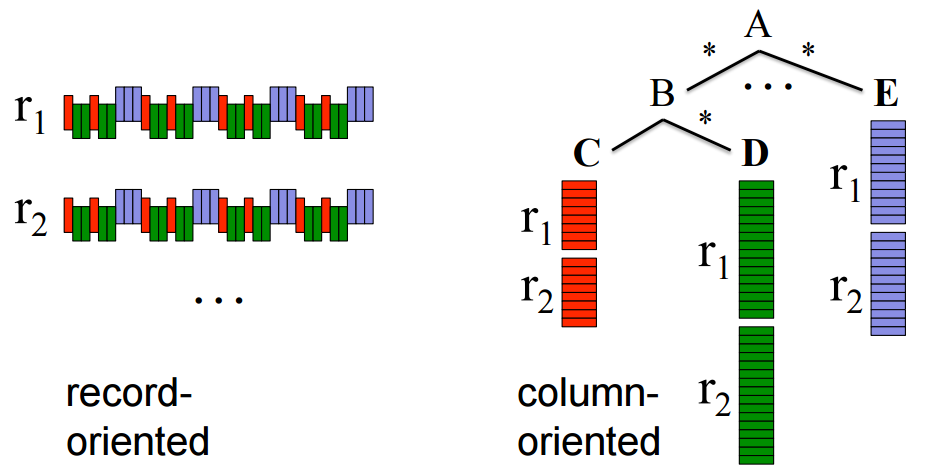
\includegraphics[width=\linewidth]{columnar.png}
\end{columns}

\vspace{0.5 cm}
I've gone back and forth on this, but now I see that Parquet's definition and repetition levels is the most elegant solution:
\begin{center}
\textcolor{blue}{\scriptsize\url{https://blog.twitter.com/2013/dremel-made-simple-with-parquet}}
\end{center}

\vspace{0.5 cm}
Each group of columns with the same multiplicity would have one ``repetition level'' array that indicates where collections and subcollections start and end. Only one repetition level array is needed for arbitrarily deep nesting: deeper repetition levels lead to higher integer values in the repetition level array. In principle, subcollections-within-collections could be as deep as $2^{64}$.
\end{frame}

\end{document}
